\documentclass[titlepage]{article}
\usepackage{graphicx}
\usepackage{multicol}
\usepackage[utf8]{inputenc}
\usepackage{authblk}
\usepackage{verbatim}
\usepackage{blindtext}
\usepackage[usenames]{color}
\usepackage{geometry}
\usepackage{hyperref}
 \geometry{
 a4paper,
 total={170mm,257mm},
 left=20mm,
 top=20mm,
 }

\usepackage[bottom]{footmisc}
\usepackage{float} % To place figures where I want them to be (with [H] option).
\usepackage{dirtytalk}
\usepackage{cancel}
\setlength{\parskip}{10px}

\usepackage{enumitem}
\usepackage{amsmath} %for using eqref
\usepackage{amssymb}
\usepackage{subfiles}

\usepackage[backend=biber, style=apa]{biblatex}
\addbibresource{bibliography.bib}
\usepackage{booktabs}
\usepackage{layouts}

\begin{document}

\title{Causal Inference - Replication Study Draft}


\author[1]{Felipe Montealegre - 1035930}

\affil[1]{Alma Mater Studiorum - Università di Bologna}

\date{March 2023}

\maketitle

%%%%%%%%%%%%%%%%%%%%%%%%%%%%%%%%%%%%%%%%%%%%%%%%%%%%%%%%%%%%%%%%%%%%%%%%%%%
\section*{Replication\footnote{Disclaimer: This is a replication exercise of Bansak and coauthors’ study on migrants' deaths and apprehensions in the US-Mexico border (\cite{Bansak2022}). Any mistakes are my own. For an accurate understanding of their study, please refer to the original article.}}

\subsection*{Technical details}

\begin{itemize}
    \item \textbf{Link to article:} \href{https://www.aeaweb.org/articles?id=10.1257/pandp.20221023}{https://www.aeaweb.org/articles?id=10.1257/pandp.20221023}.
    \item \textbf{Link to dataset and code:} \href{https://www.openicpsr.org/openicpsr/project/160201/version/V1/view}{https://www.openicpsr.org/openicpsr/project/160201/version/V1/view}.
    \item \textbf{Data and code availability:} Data and code are available for the replication study.
    \item \textbf{Code language:} STATA.
\end{itemize}

\subsection*{Context}

Every year around 100.000 people get caught illegally crossing the US-Mexico border and some 40 die trying to. The discourse of supporters for building fences revolves around an increase in security for both US citizens and migrants by deterring illegal migration. However, those who oppose this policy say that there is no decrease in migration flows nor deaths, making fence building an unnecessary expense. The Secure Fence Act (SFA), a 2006 bill from president George W. Bush authorizing and financing the construction of more fencing along the border, stoke the discussion around the benefits from doing so. The authors set up a Difference in Difference (DiD) identification strategy to identify if building fences after the SFA reduces migrant apprehensions and deaths at the border.

\subsection*{The Data}

There are 9 border sectors\footnote{From west to east along the border: San Diego, El Centro, Yuma, Tucson, El Paso, Big Bend, Del Rio, Laredo, Rio Grande Valley (See figure \ref{fig:border_sectors}). } around the US-Mexico border, and each of them is responsible for patrolling a continuous segment of the 1954 miles (3145 km) of its total extension. Each sector reports, year by year, the number of apprehensions and deaths from illegal migrants in the border (See figure \ref{fig:plot_cum_app} for a visualization of the number of apprehensions). An example of this data is in table \ref{tab:data_example_bansak} below. Note how there is no length variable as the authors arbitrarily decide which sectors are the treated ones and which are the control ones (see Identification Strategy Below).

In short: we have a panel of 9 sectors across 27 periods (1992 to 2019).

\begin{table}[h]
\centering
\caption{Example of Bansak2022 dataset}
\label{tab:data_example_bansak}
\begin{tabular}{lllllll}
sector\_number & year & sector\_name & staff & apprehensions & deaths & months80 \\
1              & 2004 & San Diego    & 1651  & 138608        & 15     & 0        \\
1              & 2005 & San Diego    & 1562  & 126904        & 23     & 0        \\
1              & 2006 & San Diego    & 1671  & 142104        & 36     & 1        \\
1              & 2007 & San Diego    & 2019  & 152460        & 15     & 0        \\
1              & 2008 & San Diego    & 2328  & 162390        & 32     & 0        \\
1              & 2009 & San Diego    & 2570  & 118721        & 15     & 0       
\end{tabular}
\end{table}

\begin{figure}[H]
\centering
    \caption{Cumulative apprehensions (millions) by sector across years.} 
    \label{fig:plot_cum_app} 
    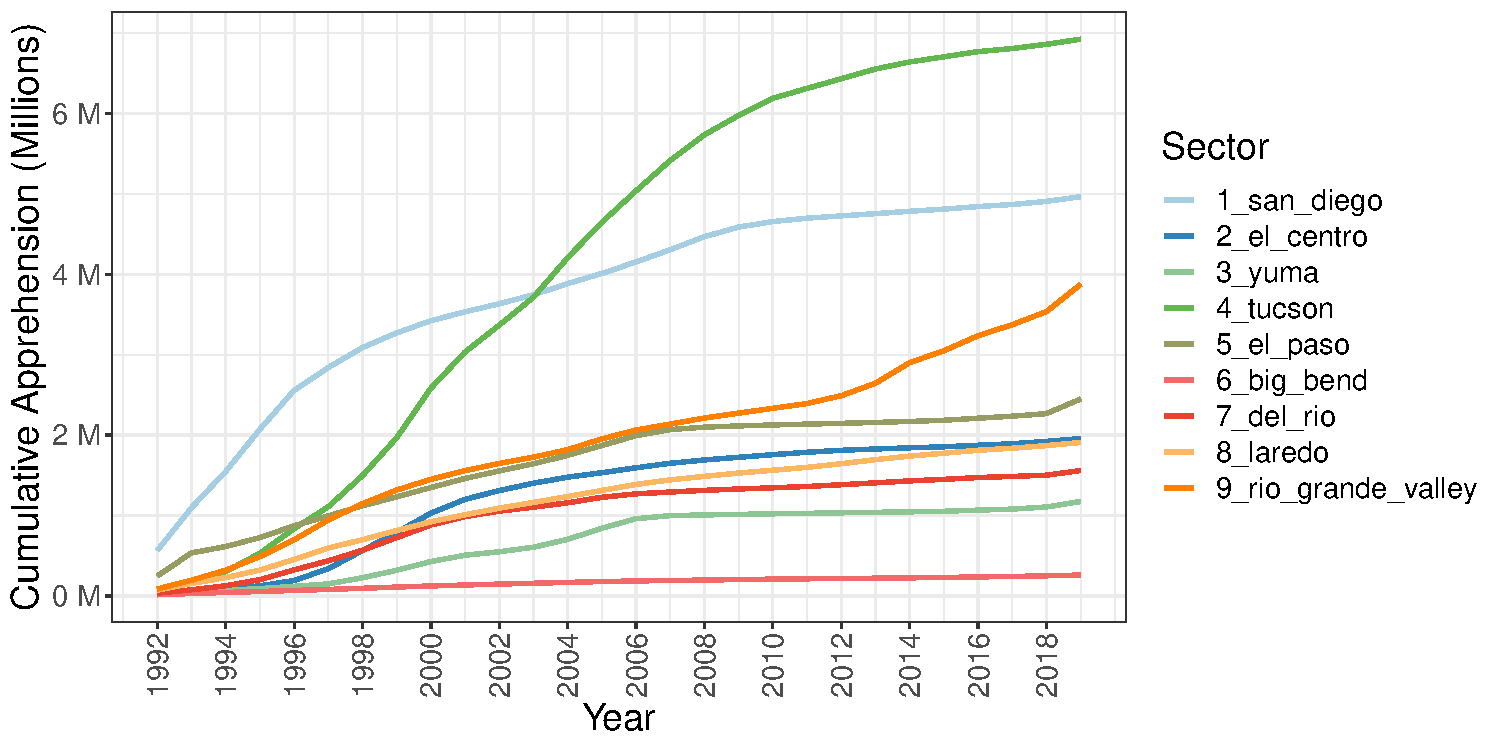
\includegraphics[width=\textwidth]{_images/plot_cum_app.pdf}
\end{figure}

\subsection*{Identification Strategy}

The authors use the following TWFE model:

\begin{equation}
    Y_{it} = \alpha + \beta_{}\textit{Fenced}_{i} + \beta_{2}\textit{SFA}_{t} + \beta_{3}\textit{Fenced}_{i} \times \textit{SFA}_{t} + \Gamma X_{it} + \epsilon_{it},
\end{equation}

where $i$ is the border sector, $t$ is the year. $Y_{it}$ represents two outcome variables: either the natural logarithm of the number of apprehensions at the border, or the ratio $(\textit{Deaths}_{it}/\textit{Apprehensions}_{it} \times 100.000)$. $\textit{Fenced}_{i}$ is an indicator equal to 1 if the  sector had new fencing constructed after passing the SFA (i.e., the treatment indicator), $\textit{SFA}_{t}$ is an indicator equal to 1 in the years after passing the SFA (i.e., the pre-post treatment indicator). $X_{it}$ is a vector of covariates including the border patrol staff and the number of months when the temperature was above $80°$ Fahrenheit. In a second specification, the authors include year fixed effects.

The authors indicate Yuma, Tucson, El Paso, San Diego, El Centro, and Rio Grande Valley, as the treated states. The control states are Big Bend, Del Rio, and Laredo. Only observations from 1998 to 2017 are included in the analysis. Years 2006 to 2008 are excluded from the analyses as fence built might be incomplete. No anticipation effects are assumed. Wall location is assumed to be exogenous (depends on environmental considerations rather than on the dependent variables).

%textwidth in cm: \printinunitsof{cm}\prntlen{\textwidth}


%%%%%%%%%%%%%%%%%%%%%%%%%%%%%%%%%%%%%%%%%%%%%%%%%%%%%%%%%%%%%%%%%%%%%%%%%%%
\section*{Extention}

\subsection*{Granular Data on Fencing Length}

I was able to prepare a data set that contains the aggregated \footnote{There are two categories of fences: Pedestrian fencing and vehicular barriers. And each of them is subdivided into primary, secondary, or tertiary depending on the existence of previously built fencing and the difficulty of crossing over the fencing. Primary fencing makes up the bulk of the built fence.} length (in miles) of fence built year by year across sectors. Merged with the authors data set I obtained a detailed description of the cumulative length of fence each sector  built year by year along with the cumulative number of apprehensions and deaths at the same level of data. Figure \ref{fig:plot_cum_length} visualizes this information. Table \ref{tab:data_example_current} shows a sample of the merged data set.

\begin{table}[]
\caption{Example of current dataset}
\label{tab:data_example_current}
\begin{tabular}{llllllllll}
sector        & year & length & cum\_len & sector\_number & staff & apprehensions & deaths & months80 & cum\_app \\
1\_san\_diego & 1998 & 9      & 35       & 1              & 2274  & 248092        & 44     & 0        & 3087449  \\
1\_san\_diego & 1999 & 2      & 37       & 1              & 2136  & 182267        & 25     & 0        & 3269716  \\
1\_san\_diego & 2000 & 3      & 40       & 1              & 2053  & 151681        & 34     & 0        & 3421397  \\
1\_san\_diego & 2001 & 0      & 40       & 1              & 2004  & 110075        & 21     & 0        & 3531472  \\
1\_san\_diego & 2002 & 0      & 40       & 1              & 1807  & 100681        & 24     & 0        & 3632153  \\
1\_san\_diego & 2003 & 0      & 40       & 1              & 1972  & 111515        & 29     & 0        & 3743668 
\end{tabular}
\end{table}

\begin{figure}[H]
\centering
    \caption{Cumulative length (miles) of built fence by sector across years.} 
    \label{fig:plot_cum_length} 
    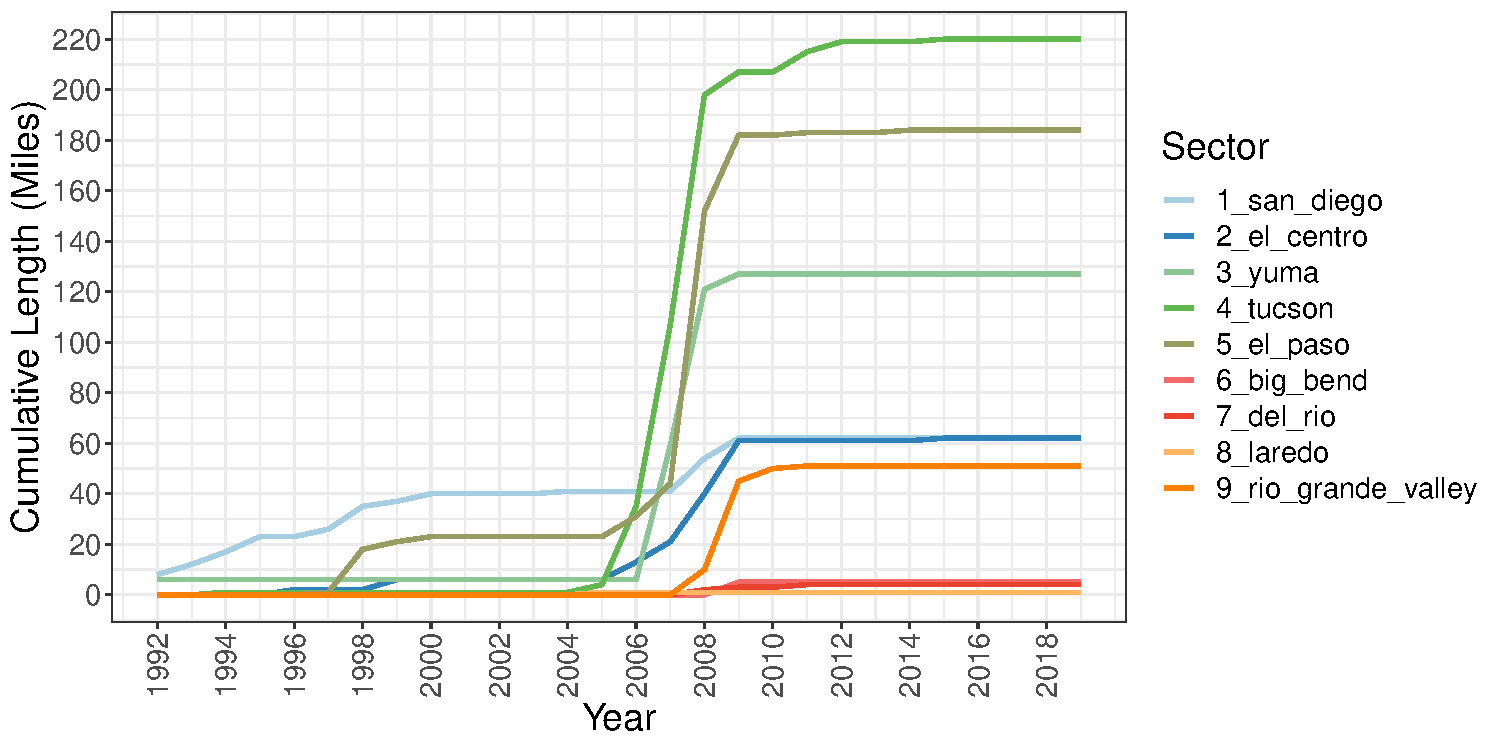
\includegraphics[width=\textwidth]{_images/plot_cum_length.pdf}
\end{figure}

\subsection*{Extension Options}

Figure \ref{fig:plot_cum_length} highlights an interesting feature of the data set: There is a component of timing in the treatment AND intensity of treatment (if we assume length of fence as the treatment variable).

\subsubsection*{Option 1: Staggered Treatment Adoption Setup.}
We could fix at 20 miles the cutoff where treatment indicator turns on. It would mean that we have 1 treated unit in 1995, 1 treated in 1998, 3 units treated in 2007, 1 in 2009, and 3 never treated. Treatment status remains on.

I followed Pedro Sant'Anna's zoom workshop you shared with us and from what I understood, it might be applied in principle. A huge doubt is sample size. Because there are the slides from Sant'Anna and a discussion in the Mixtape, I believe this is the more feasible approach for the exam.

The TWFE estimation equation would be:

\begin{equation}
    Y_{it} = \alpha_{i} + \alpha_{t} + \beta \textcolor{red}{D_{it}} + \epsilon_{it},
\end{equation}

where \textcolor{red}{$D_{it}$} is an indicator for unit $i$ being treated in period $t$.

\subsubsection*{Option 2: Continuous Treatment + Staggered Treatment Setup.}

Option 2: There is a paper from Callaway \cite{callaway2021differenceindifferences} that allows for continuous treatment AND variation in treatment timing. I tried giving it a look and the introduction of the "causal response" parameter in addition to the usual "treatment effects" left me confused; it looks quite advanced. Because this is what I think we have in the data set, it would be great to use this approach with enough time for the thesis.

Callaway's specification is:

\begin{equation}
    Y_{it} = \theta_{t} + \eta_{i} + \beta^{\textit{twfe}} \times \textcolor{red}{D_{i}} \times \textit{Post}_{t} + \upsilon_{it},
\end{equation}

where $\theta_{t}$ are time fixed effects, $\eta_{i}$ are individual fixed effects, and \textcolor{red}{$D_{i}$} is unit $i$'s dose or treatment intensity, and $Post_{t}$ is a post-treatment period dummy.


\newpage
\printbibliography[
heading=bibintoc,
title={References}]

%%%%%%%%%%%%%%%%%%%%%%%%%%%%%%%%%%%%%%%%%%%%%%%%%%%%%%%%%%%%%%%%%%%%%%%%%%%

\appendix
\addcontentsline{toc}{section}{Annexes}
\section*{Annexes}

\section{Desktop review}

\begin{itemize}
    \item Original article on KPBS from Leo Castañeda and Jean Guerrero containing detail discussion of the context of the wall, and the construction of the detailed dataset including deaths, apprehensions, miles of border constructed, by year and by sector is at \newline \href{https://www.kpbs.org/news/border-immigration/2017/11/13/americas-wall}{https://www.kpbs.org/news/border-immigration/2017/11/13/americas-wall}.
\end{itemize}

\section{Border Sectors}
Image obtained from \href{https://www.reddit.com/r/MapPorn/comments/xqku83/map_of_southwestern_border_of_the_us_with_mexico/}{link}.

\begin{figure}[H]
\centering
    \caption{Border sectors along the US-Mexico border.} 
    \label{fig:border_sectors} 
    \includegraphics[width=\textwidth]{_images/border_sectors.pdf}
\end{figure}

\section{DiD Advances and Materials}

\begin{itemize}
    \item \cite{callaway2021differenceindifferences} paper on DiD with continuous treatments: \href{https://arxiv.org/abs/2107.02637}{https://arxiv.org/abs/2107.02637}.
    \item \cite{callaway2021differenceindifferences} reading group video:
    \href{https://youtu.be/mbEJuCFCgXo}{https://youtu.be/mbEJuCFCgXo}, and its slides: \href{https://bcallaway11.github.io/files/DID-Continuous-Treatment/slides/did_reading_group.html#1}{link}
    \item \cite{callaway2021differenceindifferences} 5 minute summary: \href{https://bcallaway11.github.io/posts/five-minute-did-continuous-treatment}{https://bcallaway11.github.io/posts/five-minute-did-continuous-treatment}.
    \item \cite{Callaway2021} paper on DiD with multiple time periods. \href{https://www.sciencedirect.com/science/article/abs/pii/S0304407620303948?via%3Dihub}{link}.
    \item \cite{Callaway2021} code: \href{https://bcallaway11.github.io/did/}{https://bcallaway11.github.io/did/}
    
\end{itemize}

\end{document}


